\documentclass[8pt,notitlepage]{extarticle}
\usepackage{extsizes}
\usepackage{graphicx}
\usepackage{caption}
\usepackage{verbatim}

\title{\vspace{-30mm}Correlation between temperature of adjacent years in the 20th century in Florida, USA}
\author{Dongxuan Zhu}
\date{06/12/2022}

\begin{document}
  \maketitle
  %\begin{comment}
    \section{Materials \& Methods}

    \par This report analyzes and validates the correlation coefficient between temperatures of adjacent years \
    from an annual temperature dataset from Key West in Florida, USA for the 20th century.  
    \par In order to understand if temperatures of adjacent years have significant correlation instead of \
    correlation induced by chance alone, both correlation coefficient and permutation test are involved\
    in this analysis.
    \par To calculate correlation coefficient, the cor() package in R is used, with Pearson correlation\
    coefficient by default.
    \par In the permutation test, null hypothesis assumes the correlation coefficient is completely induced\
    by chance alone, which means there is no correlation between temperatures of adjacent years. Permutation\
    test is completed through repeated correlation calculation with randomly shuffled\
    temperature from year 1901 to 1999 with temperature from 1902 to 2000 in order. Shuffling is repeated for 10000 times to ensure sufficient\
    randomness. Afterwards, a p-value is calculated with the following formula to validate the null hypothesis:

    
    \begin{equation}
      p = \frac{\Sigma(\hat{t_{cor}})+1}{N}
    \end{equation}
    (\textbf{$\hat{t_{cor}}$}: correlation coefficients when absolute value from permutations is no smaller than absolute value from observations;\\
    \textbf{N}: repetition times)
  %\end{comment}
  
  \section{Results}

  \par The histogram shows the correlation coefficient based on permulated "first-year" temperature and "next-year" temperature in order (Figure 1), which shows a normal distribution\
  centering 0 and spreading from -0.4 to 0.3 with standard deviation atis significantly different from the observed correlation coefficient 0.3262. By calculating p-value with the above formula, a\
  small p = 1e-04 is obtained. The low p value overturns the null hypothesis, indicating that the observed correlation is not a result by chance, but\
  induced by the correlation between adjacent annual temperatures. Therefore, it is validated that temperatures of one year
  significantly correlated with the next year in the 20th century of Florida.

  \begin{figure}[h!]
    \centering
    \graphicspath{ {../data} }
    \DeclareGraphicsExtensions{.png}
    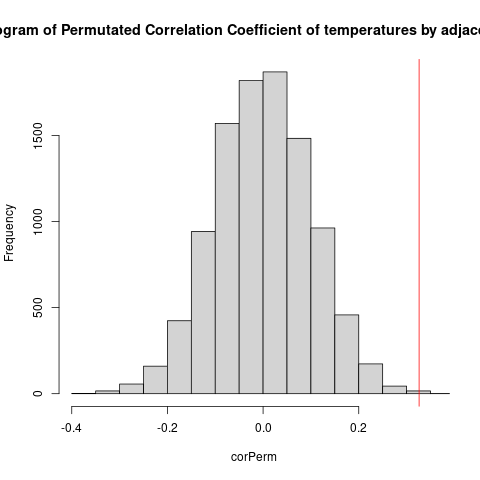
\includegraphics[width=0.4\textwidth]{PermutationTest.png}
    \caption{Comparing observed(red line) and permutated correlation coefficient value}
    \label{fig:my_label}
  \end{figure}




\end{document}